
\newcommand{\sumnat}[1]{\sum_{n=0}^{#1-1}}
\newcommand{\sumn}{\sumnat{N}}
\newcommand{\sumnn}{\sumnat{N/2}}
\newcommand{\dft}{\sumn x(n) \wn{kn}}
\newcommand{\wn}[1]{W_N^{#1}}
\newcommand{\wnn}[1]{W_{N/2}^{#1}}
\newcommand{\fn}{F_N}
\newcommand{\fnn}{F_{N/2}}
\newcommand{\fnnodd}{F_{N/2}^{odd}}
\newcommand{\fnneven}{F_{N/2}^{even}}

\newcommand{\fnv}{\ve{F_N}}
\newcommand{\fnnv}{\ve{F_{N/2}}}
\newcommand{\fnnnv}{\ve{F_{N/2^2}}}

\newcommand{\xv}{\ve{x}}
\newcommand{\wvm}{\ve{\wn{}}}

\newcommand{\pmv}{\ve{P}}
\newcommand{\cmv}{\ve{C}}

\newcommand{\pmi}{\ve{P_i}}
\newcommand{\cmi}{\ve{C_i}}
\begin{myframe}{DFT}
\centering

\begin{align*}
x(n)&  &\qquad n=0,\dots, (N-1) \\ \\
W_N&= e^{ \frac{-2 \pi i}{ N} } \\ \\
F(k)&=\dft  &\qquad k=0,\dots,(N-1)
\end{align*}


\end{myframe}

\begin{myframe}{DFT: Computation scheme}
\centering
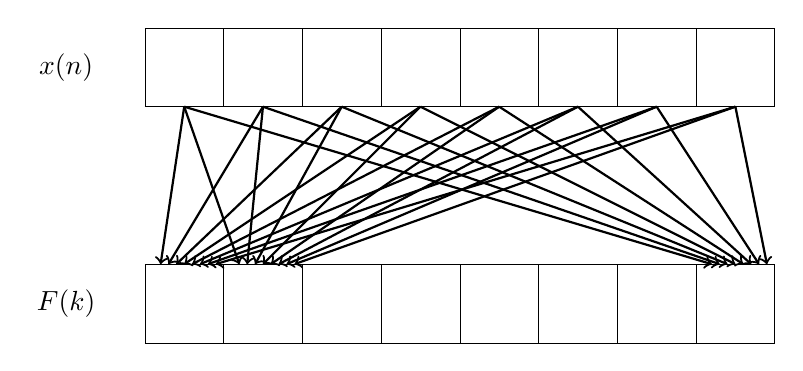
\begin{tikzpicture}[level/.style={sibling distance=60mm/#1}]

\node at (-5,1.5) {$x(n)$};
\node at (-5,-1.5) {$F(k)$};

\draw[step=1cm,very thin] (-4,-2) grid (4,-1);

\draw[step=1cm,very thin] (-4,1) grid (4,2);

\visible<1>{
\foreach \s in {0,...,7}{
    \draw[thick,->] (-3.5+\s,1) -- (-3.8+\s*0.1,-1);
}
}

\visible<2>{
\foreach \s in {0,...,7}{
    \draw[thick,->] (-3.5+\s,1) -- (-2.8+\s*0.1,-1);
}
}

\visible<3>{
\foreach \s in {0,...,7}{
    \draw[thick,->] (-3.5+\s,1) -- (3.2+\s*0.1,-1);
}
}


\end{tikzpicture}


\end{myframe}


\begin{myframe}{DFT: Implementation}
\centering
\lstinputlisting{code/dft.m}
\end{myframe}

\begin{myframe}{DFT: Time complexity}
\centering
\lstinputlisting{code/dft_time.m}
\begin{block}{}
\centering
    $O(n^2)$ operations
\end{block}

\end{myframe}

\begin{myframe}{DFT: Output}
\includegraphics[height=200pt]{img/dft}
\end{myframe}

\begin{myframe}{DFT: Properties}

\vspace{-5px}

\begin{block}{\centering $\wn{j+N/2}=-\wn{j}$}
\begin{align*}
\wn{j+N/2} &= e^{ \frac{-2 \pi i (j+N/2)}{ N} } 
           = e^{ \frac{-2 \pi i j}{ N} + \frac{-2 \pi i (N/2)}{ N} }\\
           &= e^{ \frac{-2 \pi i j}{ N}} e^{-\pi i} 
            = -\wn{j}  
\end{align*}
\end{block}

\vspace{-5px}

\begin{block}{\centering $\wn{j+N}=\wn{j}$}
\begin{align*}
\wn{j+N} &= \wn{j+N/2+N/2}  = \wn{j}
\end{align*}
\end{block}

\vspace{-5px}

\begin{block}{\centering $F(k+N)=F(k)$}
\begin{align*}
F(k+N)&= \sumn x(n) \wn{(k+N)n} = \sumn x(n) \wn{kn} \wn{Nn}\\
 &=\dft = F(k)
\end{align*}
\end{block}
\end{myframe}

